\section{Introduction}

LB method has witnessed an astonishing growth in its methodology development and application over the past quarter of a century. It fills a vital gap between the macroscopic continuum approaches such as the Navier–Stokes solvers and the particle-based microscopic approaches such as molecular dynamics. Such a mesoscopic approach has found applications in almost all areas of energy and combustion \cite{liLatticeBoltzmannMethods2016a}.

Real-time fluid simulation, i.e. the ability to simulate a virtual system as fast as the real system would evolve, can benefit to many engineering application such as the optimisation of the ventilation system design in data centres or the simulation of pollutant transport in hospitals. And although real-time fluid simulation is an active field of research in computer graphics, these are generally focused on creating visually appealing animation rather than aiming for physical accuracy. The approach taken for this thesis is different as it starts from a physics based model, the lattice Boltzmann method, and takes advantage of the computational power of a graphics processing unit (GPU) to achieve real-time compute capability while maintaining good physical accuracy. \cite{delboscRealTimeSimulationIndoor}.

turbulence modelling using the Smagorinsky model in LBM for the simu- lation of high Reynolds number flow and the coupling of two LBM simulations to simulate thermal flows under the Boussinesq approximation.

Interfaces between different phases and/or components are ubiquitous in multiphase flows and energy applications, such as rain dynamics, plant spraying, water boiling, and gas turbine blade cooling, to name but a few. A deeper understanding of the fundamental physics of such complex interfaces is of great importance in many natural and industrial processes. The dynamics of the interfaces is difficult to investigate because typical interfaces are extremely thin, complex in shape, and deforming at short time scales. In addition, the density ratio and Weber and Reynolds numbers involved in many practical multiphase flows, such as binary droplet collisions and melt-jet breakup, are usually very high, which further increases the complexity of the phenomena involved. Therefore, development of robust and accurate computational methods to capture the com- plex interfacial phenomena is crucial in the study of multiphase flows \cite{feiModelingRealisticMultiphase2019}.

During the last three decades, the mesoscopic lattice Boltzmann method (LBM), based on the kinetic theory, has become an increasingly important method for numerical simulations of multiphase flows, mainly on account of its meso-scale features, easy the numerical stability compared with the SRT-LBM. The corresponding non-orthogonal MRT-LBM has been extended to sim 

implementation, and computational efficiency.
existing multiphase LB models can be classified into four categories: the color-gradient model, the pseudopotential model, the it was shown by Li et al. that a non-orthogonal MRT-LBM free-energy model, and the mean-field model.

Among them, can retain the numerical accuracy while simplifying the implementation of its orthogonal counterpart. In parallel, the CLBM which can be viewed as a non-orthogonal MRT-LBM in the co-moving frame, has been shown to possess very good numerical stability for high Rayleigh number thermal flows,39 as well the pseudopotential model is considered in the present work due to its simplicity and computational efficiency. In this model, the interactions among populations of molecules are modeled by a density-dependent pseudopotential. Through interactions among the particles on the nearest-neighboring sites, phase separation and breakup and/or merging of phase interfaces can be achieved automatically. For further details about the multiphase LB models, interested readers are directed to some comprehensive review

\subsection{State of The Art}

To overcome difficulties of numerical instability in applying the LBM method, the multiple-relaxation-time (MRT) scheme is useful to stabilize the solution and to obtain satisfactory results because the MRT model allows the usage of an independently optimized relaxation-time for each physical process \cite{sugaD3Q27MultiplerelaxationtimeLattice2015}.

\section{Methodology}


\section{Modeling}

\subsection{Governing Equations}

The volume of fluid (VOF) model was used in this simulation. By tracking the volume fraction of each control unit, the VOF model can solve a single momen- tum equation. Thus, it can be used to simulate the fluid flow of two phase or multiphase, and it is typically applied to track the steady-state or transient gas–liquid interface.
Each phase in the model has its own volume fraction a. The sum of the volume fraction of each phase in an arbitrary calculation area is 1 \cite{lvSimulationFlowFluid2013}.

\subsection{Turbulence Modeling}

\subsection{Physical Model}
For the convenience of grid generation, the geometry of the converter in steelmaking was simplified to be cylindrical. To substitute for the converter, the cylinder with a radius of 2.0 m was used, in which the calculated depth of molten pool was 1.2 m when the mass of molten steel was 100 t.
In consideration of the geometric symmetry of the physical model with a four-hole oxygen lance, one eighth of the model as shown in Figure1 was researched.

\section{Lattice Boltzmann Method}
\label{sec:2}

The LBE is obtained by discretizing the velocity space of the Boltzmann equation into a finite number of discrete velocities $e_\alpha$ \{$\alpha$ = 0,1,...,26\}. With a proper set of discrete velocities, the LBE recovers the continuum Navier–Stokes equations by the Chapman–Enskog expansion. (It is also true for the MRT schemes.) Although many schemes to discretize the velocity space have been proposed, for three-dimensional (3-D) flows, the present study focuses on so called the three- dimensional twenty-seven (D3Q27) discrete velocity model which is illustrated in Fig. 1. Table 1 lists the sound speed $c_S$ , the discrete velocity $e_\alpha$ and the weight parameter $w_\alpha$ in the model with $c = \delta x / \delta t$ where $\delta x$ and $\delta t$ are the lattice spacing and the time step, respectively. The MRT LBM transforms the distribution function in the velocity space to the moment space by the transformation matrix $M$ . Since the moments of the distribution function correspond directly to flow quantities, the moment representation allows us to perform the relaxation processes with different relaxation-times according to different time-scales of various physical processes. The evolution equation for the particle distribution function f is thus written as

\begin{equation}
	|f (x_i +e_\alpha \delta t,t+ \delta t)\rangle-|f (x_i,t)\rangle=-M^{-1} S [|m(x_i,t)\rangle - |m^{eq} (x_i,t)\rangle]+|F(x_i,t)\rangle.
\end{equation}

where $x_i$ is the position vector of node i, $\vec{S}$ is the collision matrix, $m$ is the moment, $F$ represents an external body force and the notation for the column vector (known as the ket vector) such as $|f \rangle$ represents

%\begin{figure}[!ht]
%	\centering
%	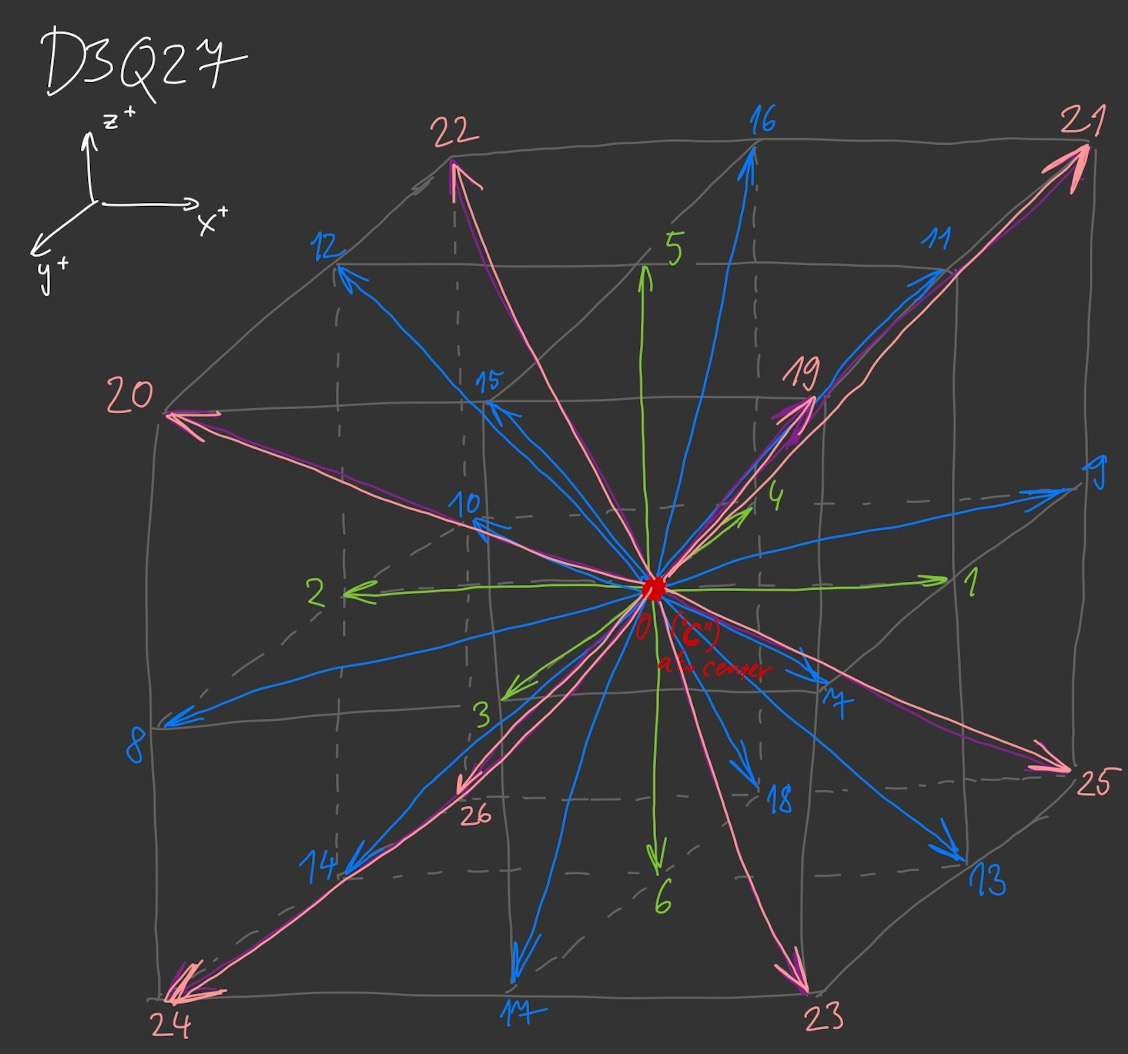
\includegraphics[width=0.4\textwidth]{figures/d3q27-bad.jpg}
%	\caption{D3Q27 node - PREROBIT NA DIAGRAM!!!}
%	\label{fig:d2q27-node}
%\end{figure}

%\begin{equation}
%|f (x_i,t)\rangle = (f_0(x_i,t),f_1(x_i,t),...,f_Q−1(x_i,t)).
%\end{equation}

\begin{equation}
	\label{eq:moments}
	\bm{m} = [m_0, m_1,...,m_{26}]^T
\end{equation}

For better numerical stability, Multiple Relaxation Time (MRT) scheme is used. It allows for more degrees of freedom and better tunability of relaxation parameters. Stability is a key property in any numerical scheme \cite{succi2001lattice}. It helps to protect against cumulative error build-up or other sources of inaccuracies.

Caution have to be taken when working within lattice's discrete world. For simulating the interface of blown oxygen with melted fluid slag, we're working with higher Mach speeds. The basic notion is that the lattice can only support signals with a finite propagation speed. Necessary criterion for stability is that physical information should not travel faster than fastest speed supported by the lattice \cite{succi2001lattice}.

We can calculate the error to $\varepsilon(Ma^3)$ in space and proportional to $\varepsilon (Ma \cdot dt)$ in time, where $Ma = \frac{u}{c_s}$ is the Mach number of the system.

$p = c_s^2 \rho$ is the pressure, $c_s = \frac{c}{\sqrt{3}}$ is the speed of sound, and the kinematic and viscosity $\nu$ is related to the relaxation time rates for the second-order moments by $\nu = \left(\frac{1}{s_v - 0.5}\right) c_s^2 \Delta t$ and $\xi = \frac{2}{3}\left(\frac{1}{s_b - 0.5}\right)$ respectively.

Transformation matrix $\bm{M}$ can be obtained from Eqs. \ref{eq:moments}.

\section{Results}

\section{Conclusions}

\section{Discussion}

